% THIS IS SIGPROC-SP.TEX - VERSION 3.1
% WORKS WITH V3.2SP OF ACM_PROC_ARTICLE-SP.CLS
% APRIL 2009
%
% It is an example file showing how to use the 'acm_proc_article-sp.cls' V3.2SP
% LaTeX2e document class file for Conference Proceedings submissions.
% ----------------------------------------------------------------------------------------------------------------
% This .tex file (and associated .cls V3.2SP) *DOES NOT* produce:
%       1) The Permission Statement
%       2) The Conference (location) Info information
%       3) The Copyright Line with ACM data
%       4) Page numbering
% ---------------------------------------------------------------------------------------------------------------
% It is an example which *does* use the .bib file (from which the .bbl file
% is produced).
% REMEMBER HOWEVER: After having produced the .bbl file,
% and prior to final submission,
% you need to 'insert'  your .bbl file into your source .tex file so as to provide
% ONE 'self-contained' source file.
%
% Questions regarding SIGS should be sent to
% Adrienne Griscti ---> griscti@acm.org
%
% Questions/suggestions regarding the guidelines, .tex and .cls files, etc. to
% Gerald Murray ---> murray@hq.acm.org
%
% For tracking purposes - this is V3.1SP - APRIL 2009
\documentclass{acm_proc_article-sp}
\usepackage{graphicx}
\usepackage{url}
\newcommand{\tup}[1]{\langle #1\rangle} 
\begin{document}

\title{Improving Live Migration: is it even worth it?}
% You need the command \numberofauthors to handle the 'placement
% and alignment' of the authors beneath the title.
%
% For aesthetic reasons, we recommend 'three authors at a time'
% i.e. three 'name/affiliation blocks' be placed beneath the title.
%
% NOTE: You are NOT restricted in how many 'rows' of
% "name/affiliations" may appear. We just ask that you restrict
% the number of 'columns' to three.
%
% Because of the available 'opening page real-estate'
% we ask you to refrain from putting more than six authors
% (two rows with three columns) beneath the article title.
% More than six makes the first-page appear very cluttered indeed.
%
% Use the \alignauthor commands to handle the names
% and affiliations for an 'aesthetic maximum' of six authors.
% Add names, affiliations, addresses for
% the seventh etc. author(s) as the argument for the
% \additionalauthors command.
% These 'additional authors' will be output/set for you
% without further effort on your part as the last section in
% the body of your article BEFORE References or any Appendices.

\numberofauthors{2} %  in this sample file, there are a *total*
% of EIGHT authors. SIX appear on the 'first-page' (for formatting
% reasons) and the remaining two appear in the \additionalauthors section.
%
\author{
% You can go ahead and credit any number of authors here,
% e.g. one 'row of three' or two rows (consisting of one row of three
% and a second row of one, two or three).
%
% The command \alignauthor (no curly braces needed) should
% precede each author name, affiliation/snail-mail address and
% e-mail address. Additionally, tag each line of
% affiliation/address with \affaddr, and tag the
% e-mail address with \email.
%
% 1st. author
\alignauthor
Zachary Estrada
\email zestrad2@illinois.edu
\alignauthor
Furquan Shaikh
\email fmshaik2@illinois.edu
}

\maketitle
\begin{abstract}
Virtualization technology is ubiquitous in most of today's datacenters and is an enabling technology for Infrastructure-as-a-Service Cloud Computing.  As the size of VM farms grows, concerns about the scalability of managing this infrastructure is growing.  Live migration techniques offer large flexibility gains at the cost of increased network traffic.  One solution to reduce this traffic involves exploiting the redundancy of data across virtual machines by migrating groups of similar virtual machines.  For this to be a worthwhile endeavor, we must first understand the nature of this redundancy.  The goal of this study is to investigate some possible use cases and determine the amount of memory redundancy that exists across VMs for these cases.  We develop a platform for evaluating this redundnacy and then utilize it to gain insight into the level of redundancy that can be exploited in these systems.
\end{abstract}

% A category with the (minimum) three required fields
%\category{H.4}{Information Systems Applications}{Miscellaneous}
%A category including the fourth, optional field follows...
%\category{D.2.8}{Software Engineering}{Metrics}[complexity measures, performance measures]
\setlength{\parindent}{0.5cm}
\section{Introduction}
Virtualization has become one of the most important technologies in today's era. It plays a crucial role in many distributed systems and services. It also forms the fundamental block in cloud computing solutions, such as Amazon EC2 \cite{ec2} and Windows Azure\cite{azure}. The reason that virtualization is widely used in such systems is that it makes better utilization of resources and reduces the cost by allowing multiple operating systems to run concurrently on the same physical infrastructure. Multiple operating systems running in their own virtual machines share the hardware resources, while ensuring high availability for the user applications \cite{virt_app}.
\par
\begin{figure}[ht]
\centering
        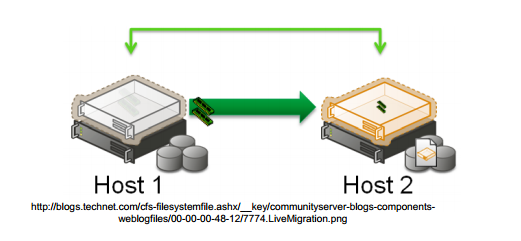
\includegraphics[height=4cm,width=9cm]{live_migration.png}
    \caption{Live Migration}
    \label{fig:live_migration}
\end{figure}
\indent With the increase in size of VM farms, scalability and manageability become a major concern. In order to solve these problems, live migration of a VM was  designed as a powerful tool. Live migration allows VMs to be reorganized for improving reachability, fault-tolerance as well as load balancing within VM farms. The basic idea of live migration is depicted in Figure \ref{fig:live_migration} \cite{live_migration}.
\par
\begin{figure*}[ht]
\centering
        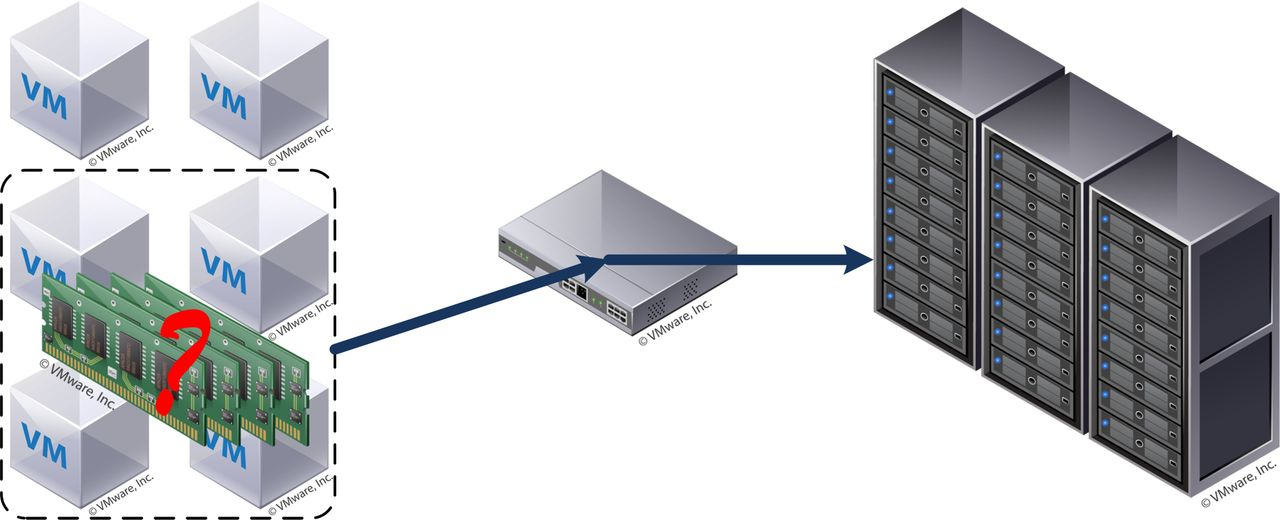
\includegraphics[height=8cm,width=18cm]{gang_migration.jpg}
    \caption{Live Gang Migration}
    \label{fig:gang_migration}
\end{figure*}
However, it is generally observed that a group of multiple VMs co-ordinate with each other in order to provide services to clients. For example, in a Map-Reduce kind of workload, the mappers and reducers are spread over a set of different VMs and all these jobs co-ordinate with each other to accomplish the goal of the user. Also, in web-server kind of environments, the web-server, database server and other servers are spread over a set of VMs in order to provide service to client requests. Thus, in order to ensure maximum performance and lower downtime for processing client requests, it is necessary to perform gang live migration of all co-ordinating VMs rather than a single live migration of individual VMs. The concept of gang live migration is shown in Figure \ref{fig:gang_migration}.
\par
Though live migration proves to be a powerful tool in increasing the manageability of the VM farms, it comes at the cost of increased network traffic. One solution to reduce this traffic is to exploit the redundancy of data across virtual machines by migrating groups of similar virtual machines. Theoretically, there exists redundant memory content across VMs in the form of kernel code, kernel static data, application libraries as well as application binaries. However, in order to ensure that the whole process of exploiting redundancy for gang live migration is worthwhile, we need to first understand the nature of this redundancy.
\par
This project aims at investigating deeper into different practical use cases and determine the amount of memory redundancy that exists across VMs for these cases. The observations and conclusions presented in this paper can be used as a guideline in deciding if it is worthwhile to invest in a distributed solution for exploiting memory redundancy for group live migration.
\par

\section{Redundancy Evaluation Architecture}\label{sec:redundancy}

\subsection{Mathematical Definition for Redundancy}\label{sec:red_math}
In this section, we intend to give a succinct definition for what is mean by memory redundancy across Virtual Machines.  In all of our analysis, we define the similarity of N virtual machines' memory as a percentage value S:
\begin{equation}
S = \frac{|(P_A \mathbf{O} P_B ... \mathbf{O} P_N|}{\sum\limits_{i=1}^{N}|P_i|}
\end{equation}\label{eqn:s}
where $P_i$ denotes the multiset of pages for VM $i$ (i.e. each element is the content of a specific page in memory) and we define the operator $\mathbf{O}$ as a sort of `intersection' of two multisets that will be clarified momentarily.  



If we let the multisets of pages be represented as sets of ordered pairs where $\tup{P,n}$ denotes that page $P$ appears $n$ times in the multiset,\footnote{The authors would like to gratefully acknowledge the help of Asaf Karagila in formalizing this definition for the operator $\mathbf{O}$.}
then we can say:
\begin{equation}\label{eqn:s}
A\mathrel{\mathbf{O}}B\equiv\{\tup{x,i+j}\mid\tup{x,i}\in A\land\tup{x,j}\in B\}.
\end{equation}
It is easy to see that since $+$ and $\land$ are associative, so is $\mathbf{O}$, and Equation \ref{eqn:s} provides the similarity fraction we wish to obtain.

The operator $\mathbf{O}$ is easily illustrated by a simple example rather than formal definition:

\begin{align*}
\textrm{Let } & A = \{1,1,2,5\},~B = \{1,2,3\}\\
\textrm{Then } &{\cal A} = \{\tup{1,2}, \tup{2,1}, \tup{5,1}\}\\
& {\cal B} = \{\tup{1,1}, \tup{2,1}, \tup{3,1}\}\\
{\cal A} \mathbf{O} {\cal B} &= \{\tup{1,3}, \tup{2,2}\} = \{1,1,1,2,2\}
\end{align*}

The example above may not be 100\% rigorous as we liberally switch between multiset and ordered pair representations, but the explanation still expresses the quantity we defined.  This metric is extremely useful when determining the amount of redundancy in a virtual machine as it quantifies the number of pages that are present across all VMs.

It should be noted than since many zero pages exist and compression techniques could be used to avoid sending these pages altogether\cite{live_adaptive_compress}, we define another metric $S_z$:
\begin{equation}
S_z = \frac{|(P_A \mathbf{O} P_B ... \mathbf{O} P_N|-N_z}{\sum\limits_{i=1}^{N}|P_i|-N_z}
\end{equation}
where $N_z$ is the total number of zero pages in all VMs:
\begin{equation}
N_z = \sum\limits_{i=1,Z\subseteq P_i}\left(|P_i\mathbf{O}Z|-1\right).
\end{equation}\label{eqn:sz}
In the equation above, $Z$ is the zero page and the $-1$ balances out the extra count we get from each $Z$ on the right-hand-side of $\mathbf{O}$.

\subsection{Implementation}\label{sec:red_implementation}
In order to compute $S$ and $S_z$ defined in the previous section, we needed to develop a framework.  A flow diagram for our measuring process is included in Figure \ref{fig:flow}.  We chose to use a Linux kernel module even though it does restrict the type of guest operating systems we can study.  However, the kernel module allowed us to test a greater variety of setups than if we had modified the hypervisor\footnote{Our current implementation, however, is restricted to the x86\_64 architecture since we use {\tt kmap()} to bring pages into virtual memory before computing the hash.  On other architectures (e.g. x86), the kernel has a concept of ``high'' memory and we cannot use the same method for calculating the hash of a physical page}(since we used testbeds involving KVM, Xen, and VirtualBox hypervisors).  Comparing the exact contents of every page in memory would require a massive amount of storage and immense computational power, so we instead used sha1 hash values for each page.  The probability of a collision is extremely low (each 1GB VM represents 262144 hash values with a 4KB page size) and the Linux kernel has a built-in crypto API,\footnote{\url{http://lxr.linux.no/linux+*/Documentation/crypto/api-intro.txt}} so we feel that this choice of hashing function has no negative impact on our results.  We standardized on 1GB VMs as much as possible, though exceptions will be noted throughout the write-up.

The process for calculating similarity is as follows (enumeration matches the flow chart in Figure \ref{fig:flow}):
\begin{enumerate}
  \item The user tells the kernel module (via a proc file)  to compute the hash of the VM's physical memory
  \item The kernel module then starts a kernel thread (kthread)
  \item The kthread iterates over the physical pages and computes the sha1 hash of every page
  \item When finished, the kernel module writes a special value to the proc file system
  \item The proc file can be polled from userspace so that the user can know when to collect the data
  \item The user starts the collection application
  \item The collection application communicates with the kernel module via a character device
  \item The saved hashes are mapped into userspace via the {\tt mmap} system call
  \item The application then reads the mapped data and outputs it to a file
  \item Another application takes the aggregated output files and selectively calculates $S$ and $S_z$ (defined in the previous Section) for the desired VM
  \item The result is obtained
\end{enumerate}
Clearly, most of these steps can be automated via simple shell scripting for semi-automated analysis.

\begin{figure}
  \centering
  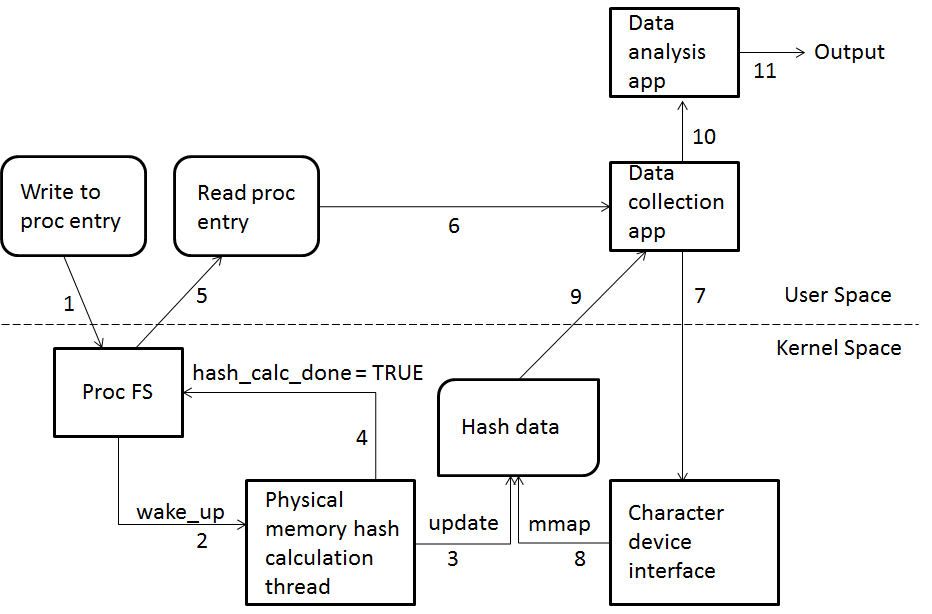
\includegraphics[width=0.4\textwidth]{images/architecture.png}
  \caption{The architecture used to calculate similarity between virtual machines}\label{fig:flow}
\end{figure}

\section{Optimistic Upper Bounds}
Before we proceed with applied use cases, we decided to get an upper bound for redundancy by testing a subset of ``ideal'' situations. This step is very important for moving ahead with the overall redundancy study because it establishes the maximum possible benefits that can be gained out of exploiting redundancy for group live migration. If the maximum value falls below the acceptable threshold, it is not worthwhile investing in sophisticated mechanisms for improving the group migration. This section describes two basic methods for establishing the optimistic upper bounds for the redundancy study.

\subsection{Same VM image across multiple instances}
This section describes the first basic method used to establish the optimistic upper bound. In this method, we used the same disk image to boot multiple cloud instances. In order to perform redundancy evaluation, every cloud instance was booted up using the common disk image followed by a snapshot of the physical memory of the VM at the end of system bootup. In this way, a total of 40VM instances were booted from the common disk image and snapshots were captured for each of the VM instances. All these snapshots were used to calculate the hash values of the entire physical memory of the VM.

\begin{figure}
  \centering
  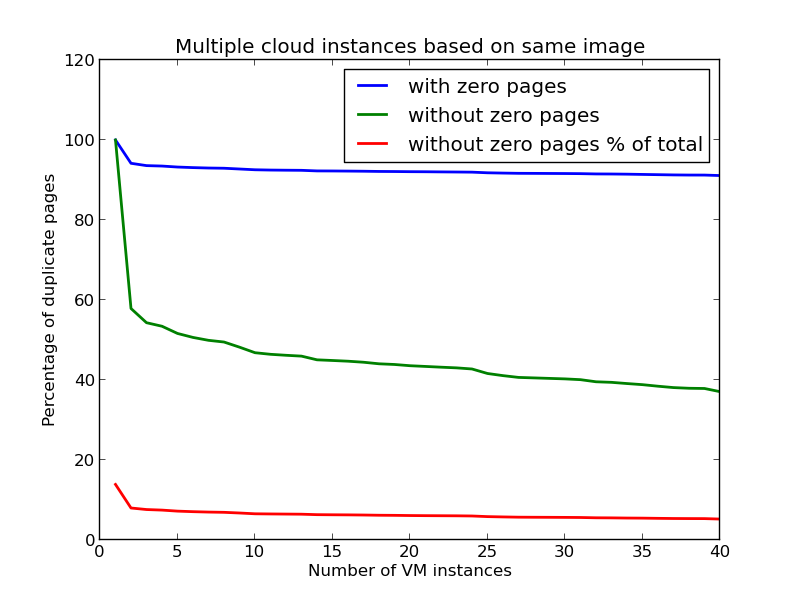
\includegraphics[width=0.4\textwidth]{images/samevm_multiplerestarts.png}
  \caption{Redundancy across multiple restarts of VMs from same image}\label{fig:multiple_restarts}
\end{figure}

Figure \ref{fig:multiple_restarts} presents the redundancy across the different VM instances. As can be seen from the figure, the amount of redundancy across different VMs including the zero pages is nearly equal to $100$\%. However, the inclusion of zero pages biases the redundancy calculation since special mechanisms like zero page compression can be used to optimize the live migration. Hence, we present two different metrics for redundancy calculation: One is the amount of duplicate memory without zero pages and other is the percentage of non-zero duplicate memory over the entire physical memory. The normalized value for non-zero duplicate memory gives the real value for optimistic upper bound on the amount of redundancy that can be achieved in the best possible case. It is clearly evident from the figure that $40$\% redundancy is the best case value for system using a common disk image to spawn multiple VMs. 


\subsection{Comparison of different variants of Linux on bootup}
This section describes the second set of experiments performed to obtain base case values for the amount of redundancy that can be exploited for group migration. In this method, we compared the redundancy that exists across different variants of Linux operating system on bootup. We used CentOS 6.4, Fedora 14, Scientific Linux 6.3 and Ubuntu 12.04 for our study.

\begin{figure}
  \centering
  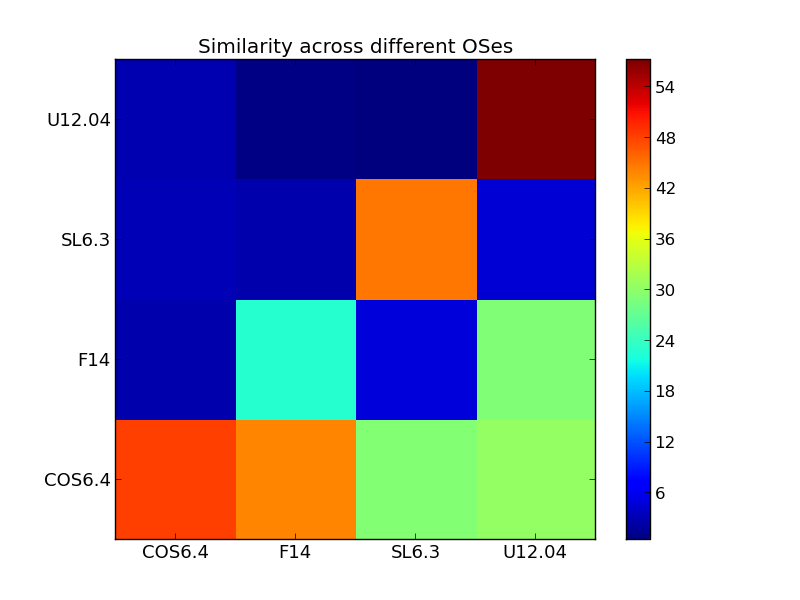
\includegraphics[width=0.4\textwidth]{images/diff_var.png}
  \caption{Redundancy across different variants of Linux}\label{fig:diff_var}
\end{figure}

Figure \ref{fig:diff_var} presents using different color codes the similarity between different variants of Linux operating system. The diagonal represents the similarity between two instances of the same operating system. The blocks below the diagonal represent the redundancy across different variants including the zero pages. On the other hand, the blocks above the diagonal, represent the redundancy not including the zero pages.

As can be seen from the figure, two different instances of the same operating system shows high similarity, nearly $30$\% to $54$\%. The similarity between different variants including zero page count ranges from nearly $18$\% to $48$\%. However, if zero pages are not considered, then the similarity across different operating systems drops down to $10$\% to $20$\%. There are the base case values that we would see with similarity only within the kernel code, since the values are captured immediately after bootup. With increase in commonality across different operating systems, this number should go on increasing.

\section{Stability Over Time}
This section presents a detailed report of the experiments performed to evaluate the stability of various systems over a period of time. We used four different systems for our study: an idle desktop system, a lightly loaded traffic server, a heavily loaded TCP client and folding at home.


\begin{figure}
  \centering
  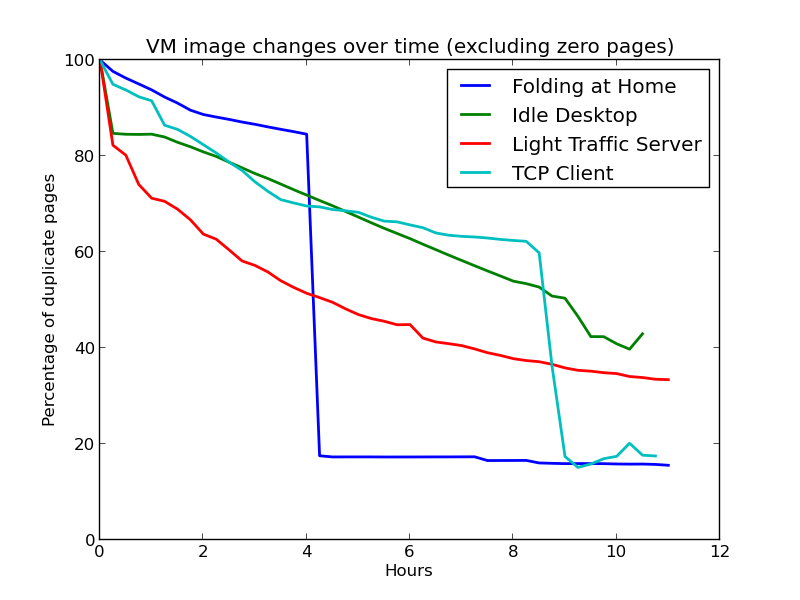
\includegraphics[width=0.4\textwidth]{images/vm_vs_time.png}
  \caption{VM image changes over time}\label{fig:vm_vs_time}
\end{figure}

Figure \ref{fig:vm_vs_time} presents the redundancy comparison of the different types of VMs discussed above over time. As can be seen from the figure, the redundancy factor within a VM seems to converge to some constant value after a certain period of time. However, the stability point that is reached by the VM varies both in time as well as in the redundancy space. Thus, within the VMs, the system memory is not constant. It keeps changing continuously. Hence, over time the trend-line shows a gradually downward progression. But, this behavior cannot be modeled using a common equation for different kinds of VMs. For example, in the lightly loaded TCP client, there are multiple points of stability and steep drop as well. On the other hand, for an idle desktop, the drop is rather gradual. Hence, depending upon the kind of applications running on the system, the overall stability changes in different ways.

\section{Client-Server}
This section describes the details of the experiments performed using a client-server kind of architecture in order to identify the level of redundancy that can be exploited during live migration. We have chosen client-server kind of use case because it well suits the model of servers deployed over a set of VMs interacting with each other to service client requests.

\subsection{Experimental Setup}
The entire group of client-server machines was realized using a set of five VMs running Ubuntu 12.04. One VM hosted the server machine, whereas the other 4 VMs hosted the client machines. In order to generate different streams of traffic, we used the standard tool Ostinato \cite{ostinato}.

The tool Ostinato has two components: First component is ostinato, which runs on the server machine and allows the server to control various ports at the server side as well as on the client side. Second component is drone, which runs on the client machines and interacts with the ostinato component on server to control different traffic streams on the client side. We used ostinato to generate random TCP traffic streams from the server to each of the clients. The data packets generated for these traffic streams were created in a completely random fashion. Also, we initiated random UDP traffic streams from each of the client machines to the server machine. Again, the data packets generated for these traffic streams were created in a completely random fashion. Overall, there were two traffic streams live at any given moment between each client-server pair(TCP downstream, UDP upstream).

\subsection{Results and Analysis}
We used the redundancy evaluation architecture to capture redundancy results along two dimensions. One is by varying the number of clients from one to four and other is by capturing the system redundancy numbers at different time instances.

\begin{figure}[htbp]
\centering
        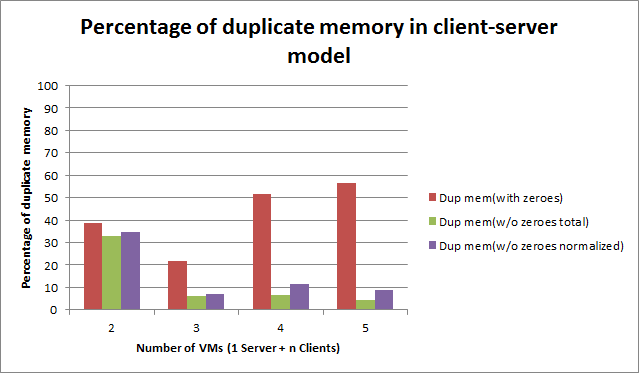
\includegraphics[width=0.4\textwidth]{client-server1.png}
    \caption{Duplicate memory with varying number of clients}
    \label{fig:client-server1}
\end{figure}

Figure \ref{fig:client-server1} presents the results of redundancy evaluation captured by varying the number of clients from one to four. Thus, the total number of VMs involved in the redundancy calculation varies from two to five. As can be seen from the above figure, the number of duplicate pages including the zero pages in the entire system is around $30$\% - $55$\%.	However, since this number includes the zero page count as well, it does not present a true indication of redundancy. Zero pages can generally be handled in a special way using compression during the process of live migration. Hence, in order to identify true redundancy, we calcuated the amount of duplicated memory without zero pages. Using these metrics, it can be seen from the figure that the amount of redundancy across the system is at least $10$\%. As mentioned in the experimental setup, the data streams between the server and the clients were made up of completely random data. Hence, the numbers that we see for redundancy are purely the lower bound on the amount of duplicate memory that can be found in a client-server architecture. With servers and clients sharing more of computational data, the amount of redundancy should go on increasing.

\begin{figure}[htbp]
\centering
        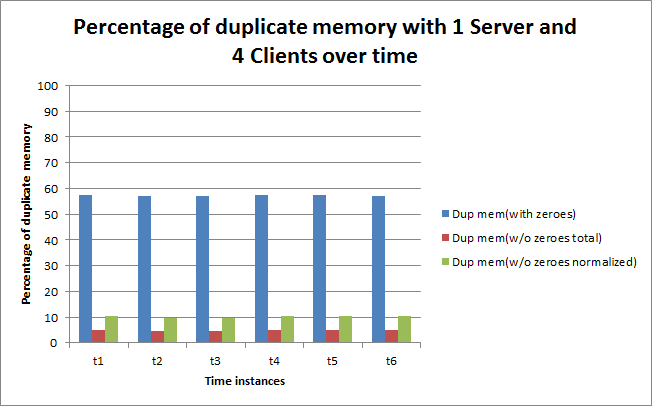
\includegraphics[width=8cm]{client-server2.png}
    \caption{Duplicate memory within the system at different time instances}
    \label{fig:client-server2}
\end{figure}

Figure \ref{fig:client-server2} present the results of redundancy evaluation captured for a system with five VMs(four clients and one server) at time instances of 30 minutes apart. As can be seen from the figure, the values for redundancy across the system at different time instances remains almost the same for duplicate memory with and without zero pages under consideration. Two conclusions can be derived from this behavior. One is that the system preferred using hot cache pages more than allocating new pages for assembling packets in memory. Hence, the total number of duplicate pages including zero pages remains almost the same. Second is that the amount of duplicate memory without zero pages remains almost the same and is at least $10$\%. This verifies our initial assumption that this number forms the lower bound on the amount of redudancy that can be exploited with completely random data running across the VMs. As the application level commonality increases in the form of data and/or code, the amount of overall system redundancy that can be exploited also increases.
\section{Hadoop}

\section{Stability Over Time}

\section{Conclusions}

\bibliographystyle{abbrv}
\bibliography{cs598mcc_paper}

\end{document}
